% This is LLNCS.DEM the demonstration file of
% the LaTeX macro package from Springer-Verlag
% for Lecture Notes in Computer Science,
% version 2.4 for LaTeX2e as of 16. April 2010
%
\documentclass{llncs}

\usepackage{amsmath}
\usepackage{amsfonts}
\usepackage{latexsym}
\usepackage{graphicx}
\usepackage{hyperref}
\usepackage{wrapfig}
\usepackage{scalefnt}
\usepackage{tikz}
\usepackage{url}
\usepackage{makeidx}  % allows for indexgeneration
%
\newcommand{\icon}[1]{\tikz[baseline=-3pt] \node[inner sep=0pt,outer sep=0pt]{\includegraphics[height=1.1em]{images/#1}};}

\begin{document}
%
\frontmatter          % for the preliminaries
%
\pagestyle{headings}  % switches on printing of running heads
%
\mainmatter              % start of the contributions
%
\title{Scientific workflow management with ADAMS}
%
\titlerunning{ADAMS: scientific workflow}  % abbreviated title (for running head)
%                                     also used for the TOC unless
%                                     \toctitle is used
%
\author{Peter Reutemann\inst{1} \and Joaquin Vanschoren\inst{2}}
%
\authorrunning{Joaquin Vanschoren et al.} % abbreviated author list (for running head)
%
%%%% list of authors for the TOC (use if author list has to be modified)
\tocauthor{Peter Reutemann and Joaquin Vanschoren}
%
\institute{University of Waikato, Hamilton, NZ, \email{fracpete@waikato.ac.nz}
\and
Leiden University, Leiden, NL, \email{joaquin@liacs.nl}}

\maketitle              % typeset the title of the contribution

\begin{abstract}
We demonstrate the practical use of a novel, flexible workflow engine, the Advanced Data mining And Machine learning System (ADAMS), designed for rapid prototyping and easy maintanance of complex knowledge workflows. Compared to most current workflow engines, ADAMS does not require the user to manually connect inputs to outputs on a large canvas. It uses a novel, compact workflow representation, \emph{control operators}, and a simple interface between operators, allowing them to be auto-connected. Moreover, it contains an extensive library of operators for various types of analysis, and a convenient plug-in architecture to easily add new ones.
\keywords{scientific workflows, machine learning, data mining}
\end{abstract}
%
\section{Introduction}
Many of today's data mining platforms offer \emph{workflow engines} allowing the user to design and run knowledge workflows, from cleaning raw data to building models and making predictions. Most of these systems, such as Kepler \cite{kepler}, RapidMiner \cite{rm} and KNIME \cite{knime2007}, are data-driven, meaning that data is passed from one operator to the next, and they represent these dependencies in a directed graph.\footnote{For an in-depth overview and comparison of scientific workflow systems, see \cite{deelman,bowers}.} Many of them take a ``canvas''-based approach, in which the user places operators on a large canvas and then connects the various inputs and outputs manually, thus introducing each dependency as a line on the canvas. 

Though this is a very intuitive approach that greatly appeals to many end users, it is also a very time consuming one. When inserting additional operators, one has to move and rearrange the entire workflow to keep the design tidy. If an operator is replaced, all connections have to be redrawn. Moreover, scientific workflows often grow very complex, including hundreds of independent steps \cite{bowers}. On a canvas, this leads to very large and complex graphs with many interconnections. This means that oversight is easily lost, even with useful features such as zooming, hierarchical workflows or meta-operators with internal workflows.

In this paper, we present ADAMS (Advanced Data mining And Machine learning System), a novel workflow engine specifically designed for rapid prototyping of complex scientific workflows, taking away the need to manually lay out and connect operators on a canvas. It presents the workflow in a compact tree structure in which operators can quickly be dragged in or pulled out, and auto-connected to the surrounding operators. It includes an extensive library of operators, including a range of \emph{control operators} to create and direct sub-flows. Moreover, new operators can be added very easily, either by dropping them in a folder, or writing them on-the-fly, without compilation, in scripts.

%In the remainder of this paper, we will first discuss ADAMS' novel workflow representation in Section \ref{representation}. After that, we briefly discuss the plug-in architecture for operators in Section \ref{newactors}. Section \ref{examples} discusses some real-world applications where ADAMS is being used, and Section \ref{conclusions} concludes.

%that uses much more compact and simplified workflow representation to allow the user to focus on quick prototyping

\section{Workflow representation}
\label{representation}

\begin{wrapfigure}{lt}{6cm}
  \centering
  \vspace{-25pt}
  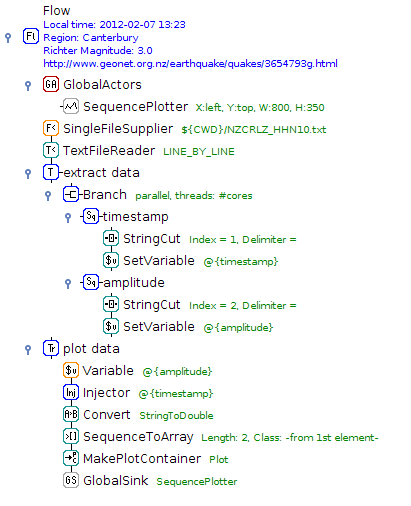
\includegraphics[width=6cm]{images/geonet_flow.png}
  \vspace{-20pt}
  \caption{An ADAMS flow.}
  \label{flow}
  \vspace{-20pt}
\end{wrapfigure}

Figure \ref{flow} illustrates an ADAMS workflow. It reads a file with earthquake data and plots it.\footnote{Simpler flows exist. This workflow is designed to explain ADAMS' control actors.} Operators (called `actors') are dragged from a library into the flow, and will automatically `snap' into the tree structure depending on where they are dropped. Actors are shown as nodes with a name and a list of parameter settings (options). They are color-coded based on whether they are a \emph{source} (only output, e.g. \texttt{SingleFileSupplier}~\icon{source}), \emph{transformer} (input and output, e.g. \texttt{StringCut}~\icon{stringcut}), \emph{sink} (only input, e.g. \texttt{SequencePlotter}~\icon{sink}) or \emph{standalone} (no in/output, e.g. \texttt{GlobalActors}~\icon{standalone}). Branches can be collapsed, and clicking actors opens a settings dialog. Some actors are fine-grained, allowing data to be manipulated within the flow, instead of requiring new actors.

\paragraph{Tokens.} Data are passed as \emph{tokens} wrapping a single Java object (e.g. a string or an entire dataset), as well as provenance information: a trace of actors affecting the data. Tokens can assume any level of granularity: actors can receive a single token (e.g., a dataset) and emit many (e.g., data points), or vice versa, buffer tokens and emit an array (e.g., the \texttt{SequenceToArray} actor). Actors with several outputs can attach a key to each token, creating a key-value pair. Many such pairs can be combined in a \emph{container}, and other actors can extract tokens based on their keys. For instance, \texttt{MakePlotContainer} attaches `X' and `Y' keys so that data can be plotted.

\paragraph{Control actors} can branch or merge sub-flows and define how data is passed between their sub-actors. \texttt{Sequence} \icon{sequence} executes its sub-actors in sequence, passing tokens from one to the next. \texttt{Branch}~\icon{branch} forwards each received token to all underlying actors and executes them in parallel. \texttt{Tee}~\icon{tee} splits off each input token, feeds it to its sub-flow and waits until it finishes before passing the token on. \texttt{Trigger}~\icon{trigger} simply starts its sub-flow upon receiving a token (without feeding the token to its sub-flow). \texttt{Injector}~\icon{injector} passes each received token on, but also injects a new token whose value is defined as a parameter. Some actors are conditioned on the value of the received token: \texttt{ConditionalTee}~\icon{conditionaltee} runs its sub-flow only if a stated condition holds, \texttt{If-Then-Else}~\icon{if} runs one of two sub-workflows depending on a test, and \texttt{WhileLoop}~\icon{while} loops over its sub-flow as long as its condition holds.

\paragraph{N-to-M semantics.} While a tree representation cannot represent N-to-M relationships, ADAMS solves this shortcoming through \emph{variables, key-value pairs, and global actors}. String tokens can be assigned to a variable using a \texttt{SetVariable} actor (e.g., \texttt{@\{timestamp\}} in Fig.\ref{flow}), and used as an actor parameter or reintroduced elsewhere as a token by the \texttt{Variable} actor. Similarly, any object token can be stored as a key-value pair by the \texttt{SetStorageValue} actor and reintroduced by the \texttt{StorageValue} actor. Finally, actors and their sub-flows can be made global: for instance, all tokens sent to a \texttt{GlobalSink} actor are passed to the referenced global actor, as shown in Fig. \ref{flow}. The scope of variables can be limited to one specific sub-flow by using the \texttt{LocalScope} control actor.


\paragraph{Interactivity.} Actors can interact with the user when needed through dialog. For instance, they can ask the user to locate an undefined file, or display a number of results and allow the user to make a subselection before proceeding.

\section{Plug-in architecture}
\label{newactors}
ADAMS contains an extensive library of actors enabling the inclusion of techniques from many existing libraries. This includes actors for machine learning techniques, importing and exporting spreadsheets, generating graphics and PDF files and sending email. A concise overview of currently supported libraries is shown in Table \ref{table}. In addition, ADAMS has a plug-in architecture to easily add new actors. A new actor can be written as a single Java class implementing a simple API. When this file is dropped into a specific folder (icon optional), ADAMS will find it and show the actor in the workflow interface. Using one of the scripting languages, actors can be developed on-the-fly without compilation.

\begin{table}[t]
\caption{Overview of currently supported tools, available through actors.}
\begin{center}
\begin{tabular}{|l|l|}
\hline
Task & Support for \\
\hline
Machine learning & WEKA, MOA, parameter optimization, experiment generation \\
Data Streams & MOA, Twitter \\
Spreadsheets & MS Excel, ODF, CSV \\
Graphics & BMP, JPG, PNG, TIF, PDF \\
Imaging & ImageJ, JAI, ImageMagick, Gnuplot \\
Scripting & Groovy, Jython \\
Other & HTTP, FTP, SFTP, SSH, Email, tar/zip/bzip2/gzip \\
\hline
\end{tabular}
\end{center}
\label{table}
\vspace{-20pt}
\end{table}%

\section{Applications}
\label{examples}
ADAMS is being used in two practical applications involving large, complex workflows. First, Gas Chromatography Mass Spectrometry (GC-MS) is a technique used to detect concentrations of compounds of interest, but the raw, high-dimensional data produced is generally not amenable to processing with machine learning systems. Using ADAMS, effective data flows were designed to entirely automate this process \cite{holmes2010}. Second, in the InfraWatch project \cite{infrawatch}, a heterogeneous sensor network of over 150 sensors is monitoring the dynamic behavior and structural health of a highway bridge. The token-based design of ADAMS proved ideal for online processing of sensor data, and its quick workflow prototyping facilitates experimentation with novel time series analysis techniques.

\section{Conclusions}
\label{conclusion}
Most scientific workflow engines use a canvas on which operators are manually arranged and connected. While this is certainly very intuitive and appealing for many end users, it is not ideal for handling very large, complex workflows. ADAMS is a rapid prototyping workflow engine designed for researchers and practitioners dealing with large workflows. It offers a wide range of operators, a plug-in architecture to include new ones on-the-fly, and a very compact workflow representation in which operators are auto-arranged, appreciatively speeding up workflow design and maintenance. Many examples and documentation can be found on ADAMS' website: \url{https://adams.cms.waikato.ac.nz/}

%
% ---- Bibliography ----
%
\begin{thebibliography}{5}
\bibitem{kepler}
Lud\"{a}scher, B., I. Altintas, C. Berkley, D. Higgins, E. Jaeger, M. Jones, E. A. Lee, J. Tao, and Y. Zhao:
Scientific workflow management and the Kepler system.
Concurrency and Computation: Practice and Experience, 18:1039�1065 (2006).

\bibitem{rm}
Mierswa, I., M. Wurst, R. Klinkenberg, M. Scholz, and T. Euler. Yale: 
Rapid prototyping for complex data mining tasks. 
In Proceedings of the 12th ACM SIGKDD International Conference on Knowledge Discovery and Data Mining (2006).

\bibitem{knime2007}
Berthold M. R., Cebron, N., Dill, F., Gabriel, T. R., K\"{o}tter, T., Meinl, T., Ohl P., Sieb, C., Thiel, K., Wiswedel, B.:
KNIME: The Konstanz Information Miner. In \emph{Data Analysis, Machine Learning and Applications}, pp. 319-326 (2008). 

\bibitem{deelman}
Deelman, E., Gannon, D., Shields, M., Taylor, I.: Workflows and e-Science: An overview of workflow system features and capabilities. Future Generation Computer Systems 25: 528-540 (2009).

\bibitem{bowers}
Bowers, S.: Scientific Workflow, Provenance, and Data Modeling Challenges and Approaches. Data Semantics 1:19-30 (2012).

\bibitem{holmes2010}
Holmes, G., Fletcher, D., Reutemann, P.: Predicting Polycyclic Aromatic Hydrocarbon Concentrations in Soil and Water Samples. Proceedings of the International Congress on Environmental Modelling and Software (IEMSS) (2010).

\bibitem{infrawatch}
Knobbe, A., Blockeel, H., Koopman, A., Calders, T., Obladen, B., Bosma, C., Galenkamp, H., Koenders, E., and Kok, J.:
InfraWatch: Data Management of Large Systems for Monitoring Infrastructural Performance.
IDA Proceedings (2010).

\end{thebibliography}

\end{document}
